%!TEX root=main.tex
\section{Architecture}
\label{sec:architecture}

\subsection{System architecture}
\label{subsec:sysarch}

\begin{figure}
\centering
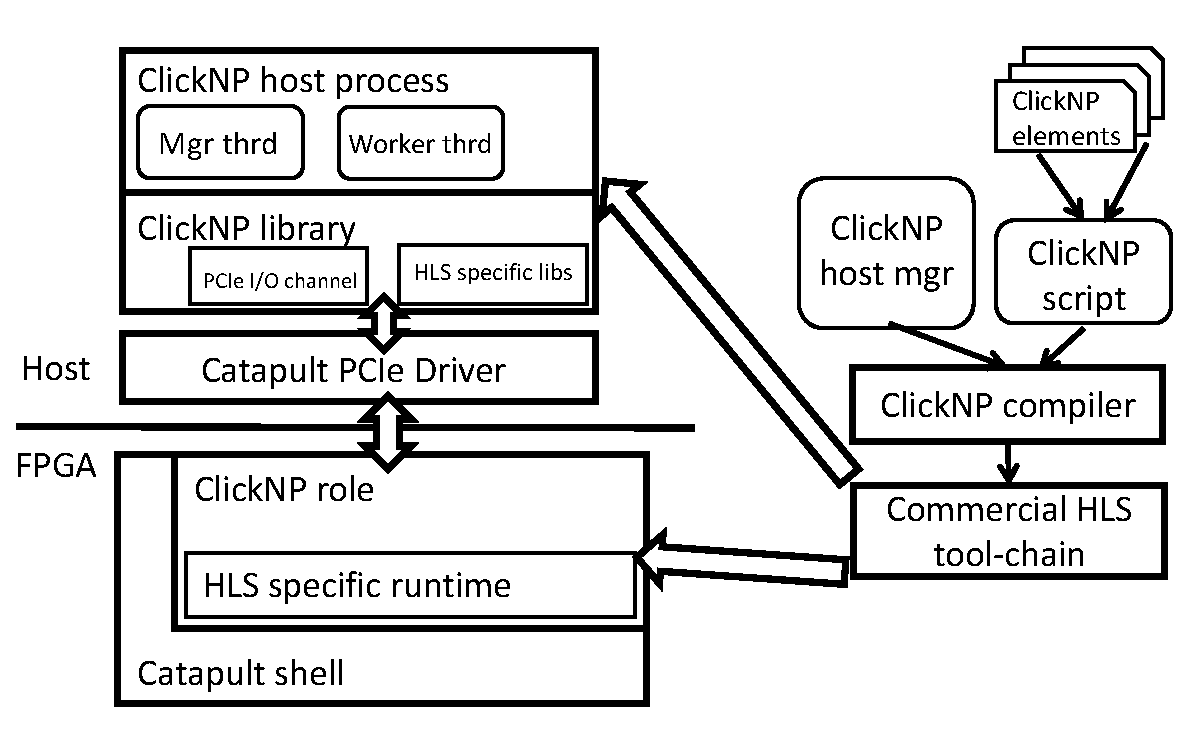
\includegraphics[width=.5\textwidth]{clicknp-arch.pdf}
\vspace{-30pt}
\caption{The architecture of ClickNP.}
\label{fig:clicknp}
\vspace{-10pt}
\end{figure}

Figure~\ref{fig:clicknp} shows the architecture of \name.
\name\ builds on the Catapult Shell architecture~\cite{putnam2014reconfigurable}.
The \textit{shell} contains many reusable bits of logic that are common for all applications 
and abstracts them into a set of well-defined interfaces,
\eg, PCIe, Direct Memory Access (DMA), DRAM Memory Manage Unit (MMU), 
and Ethernet MAC.
%
The \name\ FPGA program is synthesized as a Catapult \textit{role}.
%
However, since \name\ relies on commodity HLS tool-chains to generate FPGA HDL, 
and different tools may generate their own (and different) interfaces for the resources managed by the shell, 
we need a shim layer, called \textit{HLS-specific runtime}, to perform
translations between HLS specific interfaces to the shell interfaces. 

A \name\ host process communicates with the \name\ role through the \name\ library,
which further relies on the services in Catapult PCIe driver 
to interact with FPGA hardware.
The \name\ library implements two important functions: 
(1) It exposes a PCIe channel API to achieve high-speed and low latency communications 
between the \name\ host process and the role; 
(2) It calls several HLS specific libraries to pass initial parameters to
the modules in the role, as well as control the start/stop/reset of these 
modules.
%
The \name\ host process has one manager thread and zero or multiple 
worker threads.
%
The manager thread loads the FPGA image into the hardware, starts worker threads, 
initializes \name\ elements in both FPGA and CPU based on the configuration, 
and controls their behaviors by sending \textit{signals} to elements 
at runtime. 
%
Each worker thread may process one or more modules if they are assigned to CPU.

\subsection{\name\ programming}

\subsubsection{Abstraction}

\name\ provides a modular architecture and the basic processing module is called an \textit{element}.
A \name\ element has the following properties: 
\begin{itemize}
\item Local states. Each element can define a set of local variables that are only accessible inside the element. 
\item Input and output ports. An element can have any number of input or output ports. 
\item Handler functions. An element has three handler functions: (1) an initialization handler, which is called once when the
element starts, (2) a processing handler, which is continuously called to check input ports and process available data,
and (3) a signal handler, which receives and processes the commands (\textit{signals}) from the manager thread in the host program.
\end{itemize}

%\vspace{-6pt}
An output port of an element can connect to an input port of another element through a \textit{channel}, as shown in Figure~\ref{fig:element}(a).
In \name, a channel is basically a FIFO buffer that is written to one end and read from the other end.
The data unit of the read/write operations to a channel is called \textit{flit}, which has a fixed size of 64 bytes.
The format of a flit is shown in Figure~\ref{fig:element}(b). Each flit contains a header for meta-data and a payload of 32 bytes.
A large piece of data, \eg, a full-sized packet, is broken into multiple flits, when flowing among \name\ elements.
%Currently, we choose 32-byte data bus size, and therefor to allow up to 51.2Gbps throughput under 200MHz clock.}
The first flit is marked with \textbf{sop} (start of packet), and the last flit is marked with \textbf{eop} (end of packet). 
If the size of the data piece is not 32, the \textbf{pad} field of the last flit indicates how many bytes have been padded to the payload. 
%Reserved field in a flit is optimized out by HDL synthesis tools.
% why flit
We note that breaking large data into flits not only reduces latency, but also potentially increases parallelism as
different flits of a packet may be processed at different elements simultaneously.
%
Finally, to fulfill a network function, multiple \name\ elements can be interconnected to form a directed processing graph, which 
is called a \name\ \textit{configuration}. 

Clearly, the \name\ programming abstraction largely resembles Click software router~\cite{kohler2000click}. 
However, there are three fundamental differences which make \name\ more suitable
for FPGA implementation:
(1) In Click, edges between elements are C++ function calls and a \textit{queue} element is required to store packets.
However, in \name, an edge actually represents a FIFO buffer that can hold actual data. Additionally, \name\ channels break the data dependency among elements and allow them to run in parallel. 
%	FIFO also leverages \textit{pipe} abstraction in OpenCL for efficient hardware generation.
(2) Unlike Click, where each input/output port can be either \textit{push or pull}, 
\name\ has unified these operations: An element can only \textit{write (push)}  to any output port, while \textit{read (pull)} can do so from any input port.
%This is a more flexible model and allows elements to be reused in both ingress and egress pipeline.
(3) While Click allows an element to directly call methods of another element (via flow-based router context), in \name,
the coordination among elements is \textit{message-based}, \eg, a requester sends a request message to a responder and gets a response via another message.
%
Message-based coordination allows more parallelism and is more efficient in FPGA compared to coordination through shared memory, where accessing a shared memory location has to be serialized and would become a bottleneck.

\begin{figure}
\centering
\begin{tabular}{c}
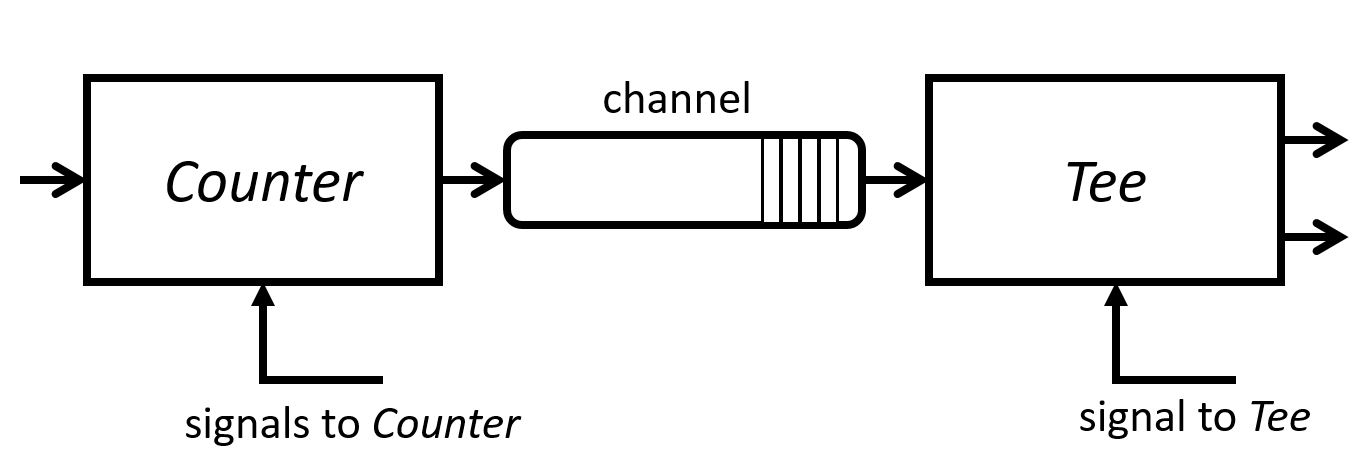
\includegraphics[width=.4\textwidth]{element.jpg} \vspace{-6pt} \\
(a)\\
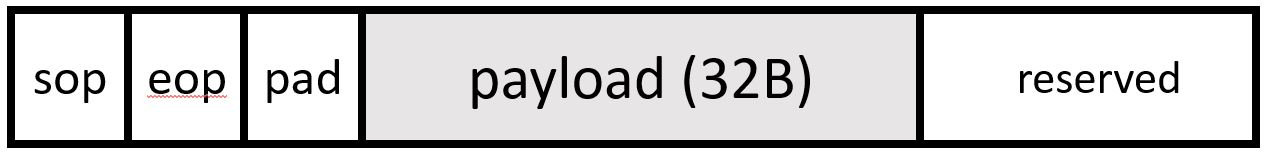
\includegraphics[width=.35\textwidth]{flit.jpg} \\
(b) \\
\end{tabular}
\vspace{-10pt}
\caption{(a) Two \name\ elements are connected through a channel. (b) The format of a flit. }
\label{fig:element}
\vspace{-17pt}
\end{figure}

\subsubsection{Language}

\name\ elements are alike objects in an object-oriented language, and can be defined using such languages, \ie, C++.
Unfortunately, many existing HLS tools support only C. 
To leverage the commercial HLS tools, we could write a compiler that converts a object-oriented language, \eg C++, to C.
But this effort is non-trivial.
In this work, we take an alternative path to extend C language to support element declaration.
Figure~\ref{fig:lang}(a) shows a code snippet of element \textit{Counter}, which simply counts how many packets have
passed. An element is defined by \textbf{.element} keyword, followed by the element name and the number of input/output ports.
The keyword \textbf{.state} defines the state variables of the element, and \textbf{.init}, \textbf{.handler}, and \textbf{.signal}
specify the initialization, processing, and signal handler functions of the element.
A set of built-in functions are implemented to operate on the input and output ports, as summarized in Table~\ref{tab:built-in}.

Similar to Click, \name\ also uses a simple script to specify a configuration of a network function. The configuration has
two parts: \textit{declarations} and \textit{connections}, following the similar syntax of Click language~\cite{kohler2000click}.
One thing worth noting is that in \name\, we can use a keyword \textbf{host} to annotate an element, which will cause 
the element to be compiled into CPU binary and executed on CPU.

\begin{table}
\vspace{-10pt}
\centering
\caption{Built-in operations on \name\ channels.}
\label{tab:built-in}
\small
\begin{tabular}{p{.2\textwidth}|p{4cm} }
\toprule \\
uint get\_input\_port() & Get bitmap of all input ports with available data. \\
\midrule
bool test\_input\_port(uint id) & Test the input port indicated by id. \\
\midrule
flit read\_input\_port(uint id) & Read the input port indicated by id. \\
\midrule
flit peek\_input\_port(uint id) & Peek input data from the port indicated by id. \\
\midrule
void set\_output\_port(uint id, flit x) & Set a flit to the output port. The flit is written to the channel when the handler returns.\\
\midrule
ClSignal read\_signal() & Read a signal from signal port.\\
\midrule
void set\_signal(ClSignal p) & Set an output signal on signal port.\\
\midrule
return (uint bitmap) & Return value of \textbf{.handler} specifies a bitmap of input port(s) to be read on next iteration. \\
\bottomrule
\end{tabular}
\vspace{-10pt}
\end{table}

\begin{figure}[t!]
\scriptsize \lstset{style=numbers}

\lstset{ emph={%
 element, init, state, handler, signal,include
}, emphstyle={\bfseries .},
morekeywords={get_input_port,read_input_port,from_tor, to_tor, set_output_port, host, set_signal} 
}
\centering
\begin{tabular}{c}

\begin{lstlisting}
element Count <1, 1> {
  state{
    ulong count;
  }
  init{
    count = 0;
  }
  handler{
    if (get_input_port() != PORT_1) {
      return (PORT_1); 
    }
    flit x;
    x = read_input_port(PORT_1);
    if (x.fd.sop) count = count + 1;
    set_output_port(PORT_1, x);
   
    return (PORT_1);
  }
  signal{
    ClSignal p;
    p.Sig.LParam[0] = count;
    set_signal(p);
  }
}
\end{lstlisting} \vspace{3pt} \\
{\normalsize \centering (a)} \vspace{3pt} \\
\begin{lstlisting}
Count :: cnt @ 
Tee :: tee 
host PktLogger :: logger

from_tor -> cnt -> tee [1] -> to_tor
tee [2] -> logger
\end{lstlisting} \vspace{3pt} \\
{\normalsize \centering (b)} 
\end{tabular}
\caption{\name\ language to write elements and specify configurations. An element annotated with \textbf{host} keyword is compiled and executed on the CPU. An element annotated with ``@'' is required to receive control signals from the manager thread. 
\textbf{``From\_tor''} and \textbf{``to\_tor''} are two built-in elements that represent input and output of an Ethernet port on FPGA. The return value of the handler function specifies
a bit-mask of input ports that will be checked in next round.}
\label{fig:lang}
\vspace{-10pt}
\end{figure}

\subsubsection{\name\ tool-chain}
\label{subsec:toolchain}
The \name\ tool-chain contains a \name\ compiler as the front-end, and a C/C++ compiler (\eg, Visual Studio or GCC) and an HLS tool 
(\eg, Altera OpenCL SDK or Xilinx Vivado HLS) as the back-end.
% Overview of ClickNP programming process
As shown in Figure~\ref{fig:clicknp}, to write a \name\ program, a developer needs to divide her code into three parts:
% very similar to the Click Modular Router~\cite{kohler2000click}:
(1) A set of elements, each of which implements a conceptually simple operation,
(2) A configuration file that specifies the connectivity among these elements,
and (3) A host manager that initialize each element and control their behavior during the runtime, \eg, according to the input of administrators.
%
These three parts of source code are fed into the \name\ compiler and translated 
into intermediate source files for both host program and FPGA program. 
The host program can be directly compiled by a normal C/C++ compiler, while the FPGA program is synthesized using commercial HLS tools.
%
Existing commercial HLS tools can determine a maximum clock frequency of 
each element through timing analysis. 
Then, the clock of a \name\ processing graph is constrained by the slowest element in the graph.
%
Additionally, HLS tools may also generate an optimization report which shows the 
dependency among the operations in an element. An element is \textit{fully pipelined}
if all dependency is resolved and the element achieves the optimal throughput by 
processing one flit in every clock cycle.

\egg{
Our ClickNP architecture is built on state-of-the-art data center reconfigurable hardware (Catapult FPGA \cite{putnam2014reconfigurable}) and FPGA programming framework (Altera OpenCL \cite{singh2011implementing}).

\subsection{Catapult FPGA}

Catapult \cite{putnam2014reconfigurable} is a reconfigurable hardware designed for offloading feature extraction, feature computation and scoring in search engine ranking. We modify the hardware to incorporate two on-board 40 GE MACs, so the FPGA can receive and send network packets via the two 40 GE ports without CPU intervention.

\begin{figure}[!t]
	\center
	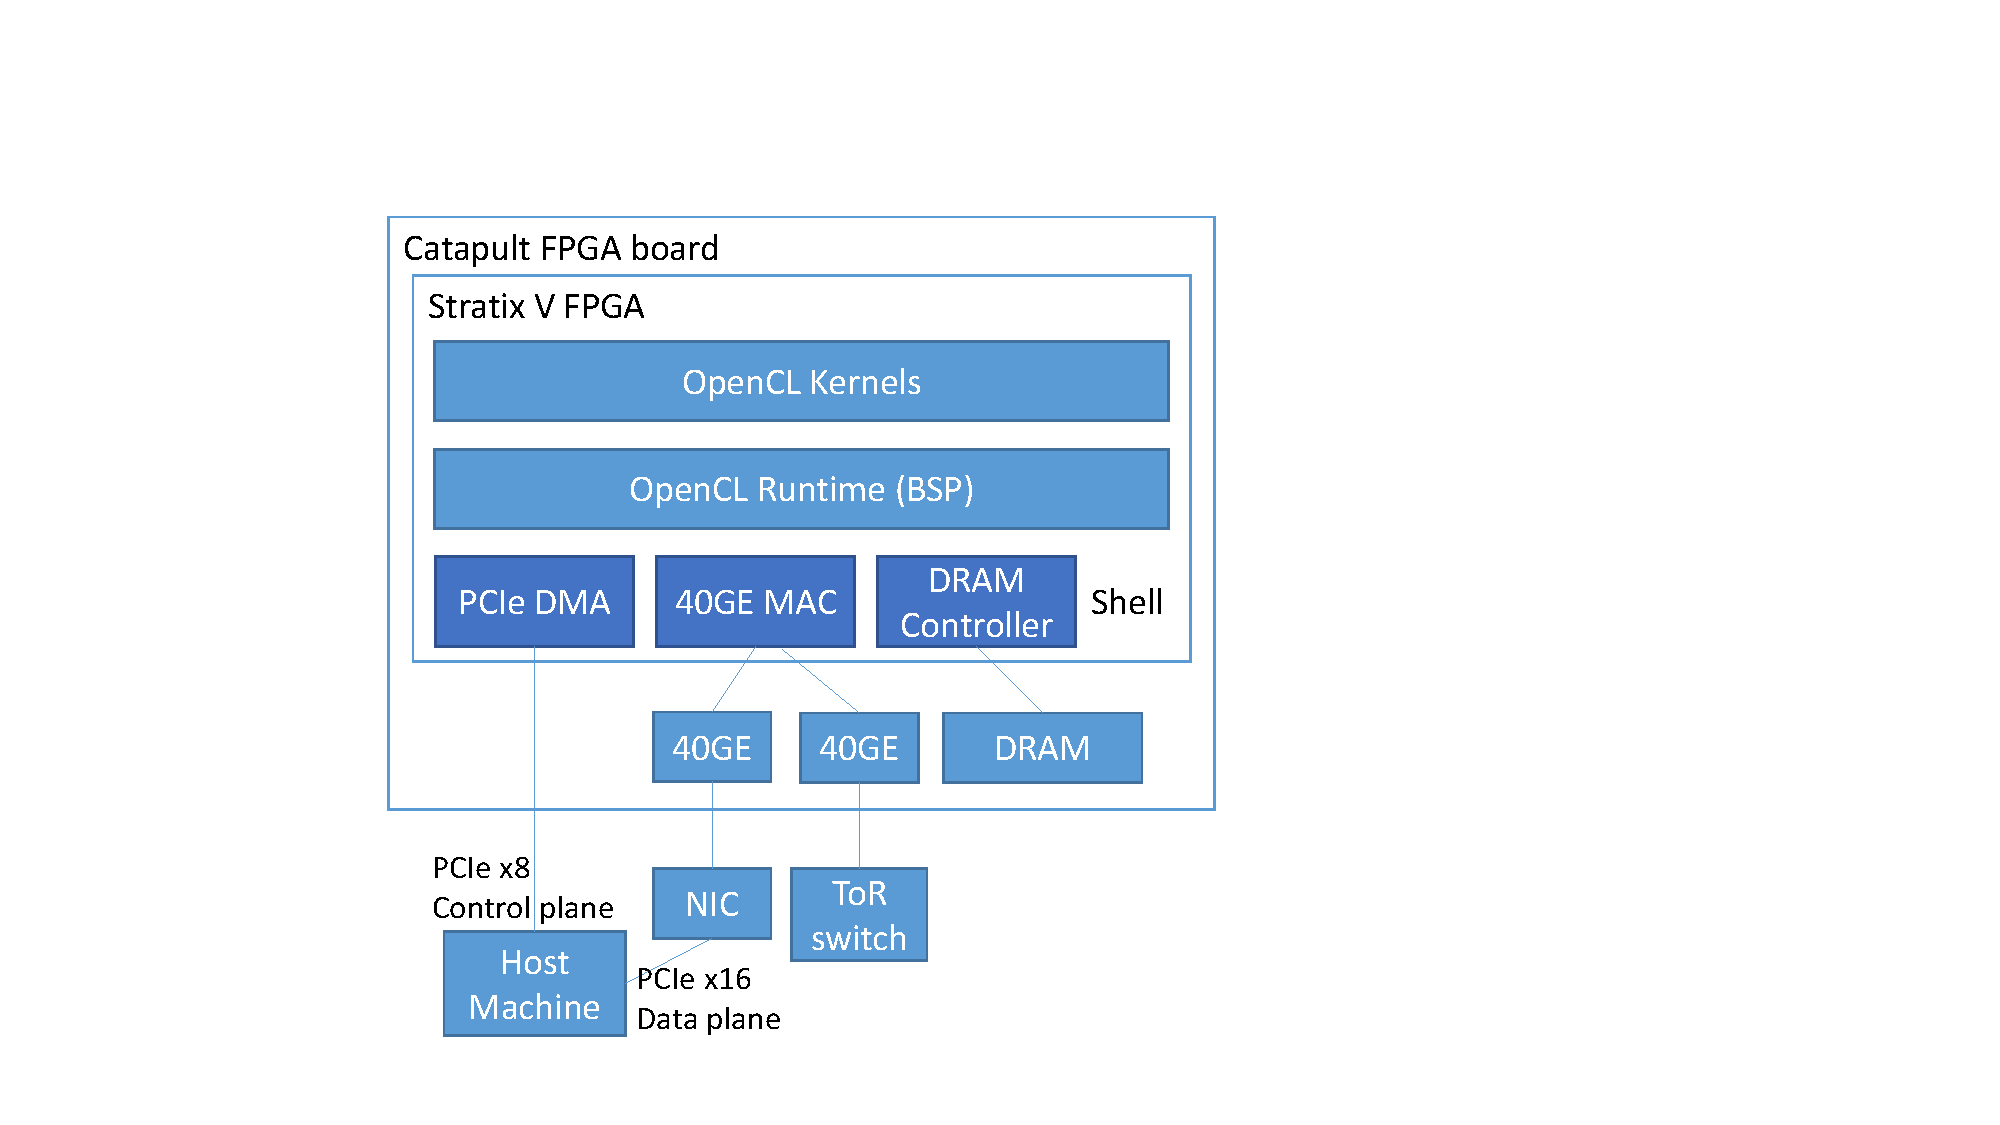
\includegraphics[width=1.0\columnwidth]{image/CatapultFPGAArch}
	\vspace{-0.25in}
	\caption{Catapult FPGA Architecture}
	\vspace{-0.15in}
	\label{fig:CatapultFPGAArch}
	%    \vspace{-2mm}
\end{figure}

In network virtualization scenario, we install one FPGA in each server and connect two 40 GE ports to NIC and Top-of-Rack (ToR) switch respectively. The traffic between NIC and ToR flow through the FPGA to perform comprehensive network functions \textit{bump-in-the-wire}, including tunnel encapsulation and decapsulation, firewall, metering and traffic scheduling. Virtual machines expose to the NIC and FPGA via Single-Root I/O Virtualization (SR-IOV), and data-plane functions of the virtual switch are offloaded to the FPGA.

Current generation of Catapult FPGA has 172,600 ALMs (Adaptive Logic Modules) each containing several 8-input configurable lookup table, two full adders and four one-bit registers \cite{alterafpgaarch}, 2,014 blocks of 20 Kbit SRAM and a 4 GB DRAM. Each register can be read and written every cycle without latency. Each SRAM block can perform one read or write operation with exactly one cycle latency. The performance of DRAM depends on access pattern. When accessed randomly, each operation takes 170 ns (about 34 cycles); when accessed sequentially, the throughput can reach 4 Gbps. Registers, SRAMs and DRAM form a memory hierarchy where faster memory spaces have lower capacity.

\subsection{OpenCL Compiler}

The Altera SDK for OpenCL \cite{singh2011implementing} is a programming framework that abstract away the traditional hardware FPGA development flow. In the OpenCL \cite{khronos2008opencl} model, data-plane functions are wrapped in \textit{kernels} and compiled into hardware accelerators, and control plane on the host machine communicates with kernels via a standard set of APIs. Altera OpenCL introduces \textit{channels} to allow communication among kernels without host intervention.

Central to Altera OpenCL is a compiler \cite{czajkowski2012opencl} that extracts parallelism in OpenCL kernels and generates Verilog code. A parser based on LLVM first parses OpenCL kernel and produces intermediate representation (IR) consisting of instructions and dependencies between them. Then the IR is optimized via live-variable analysis and generate CDFG (Control Data Flow Graph). Based on CDFG, scheduler determines the required clock cycles of each operation, then sequence the operations into a pipeline, where independent operations are parallelized and dependent operations are pipelined. Finally the compiler links to IP library and generates Verilog HDL, as well as a profiling report containing estimated resource utilization and an optimization report containing data dependencies that lead to pipeline stall.

OpenCL is designed primarily for batch processing instead of stream processing, which is a gap that ClickNP needs to bridge. In network stream processing, kernels run in an infinite loop, so the kernels will never finish.

First, when a kernel is running, global memory assigned to it cannot be accessed by the host machine. So commands can not be passed to kernels via global memory on-the-fly. One straightforward approach could be launching another ``proxy'' kernel to pass in commands via channel each time the host sends a command. However, this approach has about 5 millisecond latency due to complicated internals in launching and finishing a kernel. Fortunately, OpenCL only occupies PCIe slots 0--31, so we designed a raw I/O channel via PCIe slots 32--39 to allow on-the-fly interaction of kernels and the host. Figure \ref{fig:PCIeChannelPerf} shows that PCIe I/O channels reach near-theoretical throughput with 5 slots and 16K batch size, and the latency for small batch size is microsecond-scale.

\begin{figure}[h!]
	\centering
	\subfigure[Latency (x: batch size, y: microsec; lines: polling, interrupt, opencl)]{
		
\includegraphics[width=0.45\columnwidth]{image/logo}
		\label{fig:PCIeChannelLatency}
	}
	\subfigure[Throughput (x : number of slots; y: Gbps; lines: batch size, theory)]{
		
\includegraphics[width=0.45\columnwidth]{image/logo}
		\label{fig:PCIeChannelThroughput}
	}
	\vspace{-0.15in}
	\caption{PCIe Channel Performance}
	\vspace{-0.15in}
	\label{fig:PCIeChannelPerf}
	%    \vspace{-2mm}
\end{figure}

Second, since the kernels never finish, when the host program crashes or need to be updated, although the data plane is still running, we might lose the control plane because the kernels may have problem launching again. We added a PCIe-controlled register to trigger reset signal of OpenCL kernel programs and OpenCL runtime on FPGA. When the host program restarts, it toggles the reset register to force stop all kernels and then re-launch them via OpenCL API.

\subsection{ClickNP Toolchain}

The building blocks of ClickNP are \textit{elements}. Each element is compiled to an OpenCL single-work-item \textit{kernel}.

A ClickNP \textit{project} consists of 3 parts: a library of elements, a \textit{Click script} to specify what and how elements are connected, and a \textit{host program} to interact with the user and issue commands to elements.

ClickNP provides 4 build targets for a project:

\begin{enumerate}
	\item Native x86 emulation (in seconds) with ClickNP compiler and standard C++ compiler to test functionality and debug with \textit{printf}.
	\item Generate optimization report (in 1 minute) to understand resource utilization and memory dependencies with ClickNP compiler and OpenCL compiler. If an element is not fully pipelined, or the overall resource utilization is too high, developer should optimize the element code (if a new element is written) or change element parameters (e.g. lookup table size).
	\item Build full FPGA image (in 1--2 hours) with ClickNP compiler, OpenCL compiler and Quartus synthesizer, fitter, assembler and timing analyzer.
	\item Build host program (in seconds) with ClickNP compiler and standard C++ compiler.
\end{enumerate}

%Multiple emulation-mode ClickNP projects can be connected via named pipes, e.g. connect the traffic generator, your bump-in-the-wire ClickNP project and the traffic monitor with pipes to test functionality with various traffic patterns without code modifications.

\begin{figure}[!t]
	\centering
	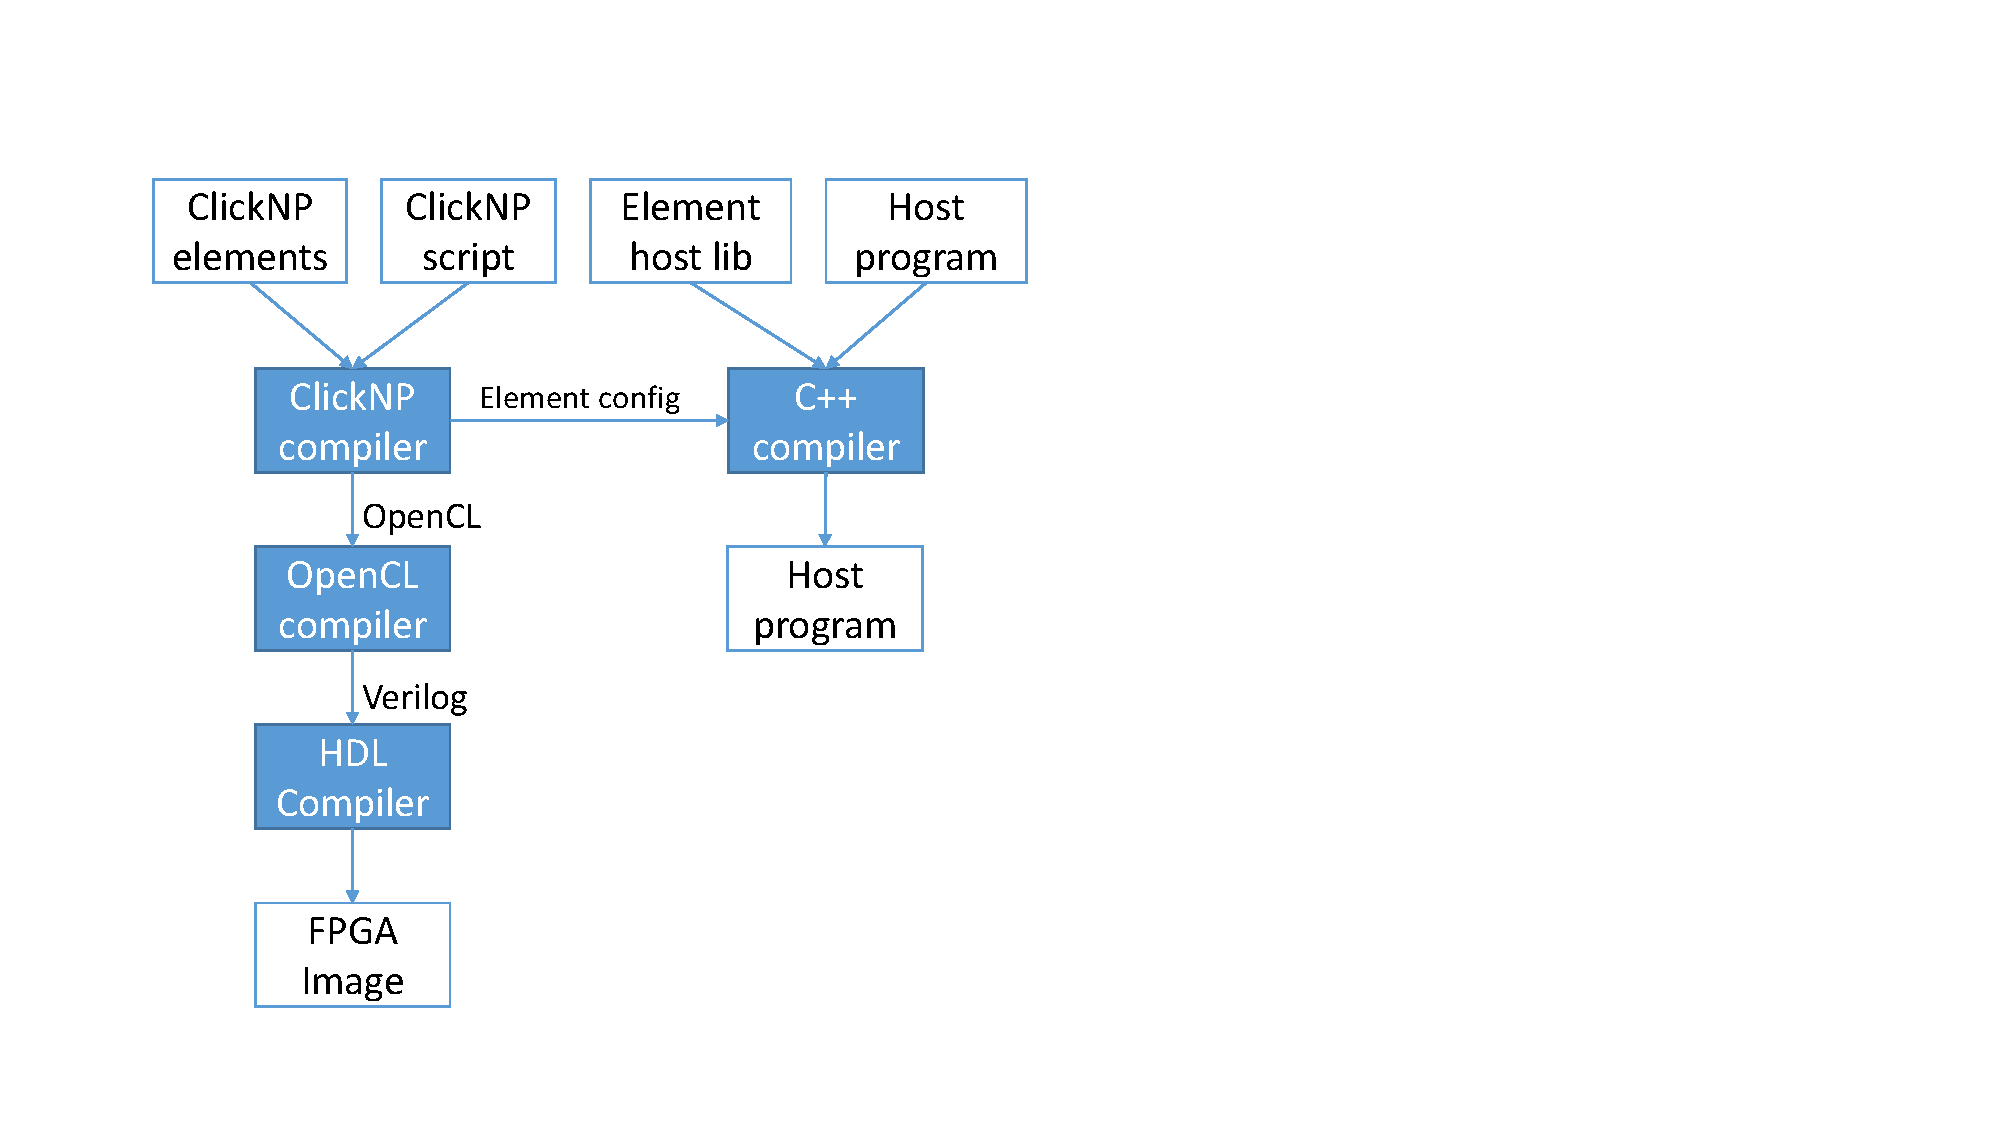
\includegraphics[width=0.8\columnwidth]{image/ClickNPSoftware}
	\vspace{-0.15in}
	\caption{ClickNP Compilation Flow}
	\vspace{-0.15in}
	\label{fig:ClickNPSoftware}
	%    \vspace{-2mm}
\end{figure}

Full compilation of a project generates an FPGA image, a x86 host program and an OpenCL kernel binary. First, the FPGA image is reprogrammed into FPGA via Flash Util in Figure \ref{fig:CatapultFPGAArch} (30 seconds). Second, the host program starts, resets the FPGA board, loads OpenCL kernel binary and launches all kernels. Then the host program keeps running, accepts control plane commands via terminal or RPC, issues signals to elements and listen to events from elements.

When the host program needs to be updated, simply kill the host program and the data plane will keep running. The new host program can choose to either re-initialize all element states, or keep the states and clear in-flight signals and events in case the host program was killed halfway in host-kernel communication.

\begin{figure}[!t]
	\centering
	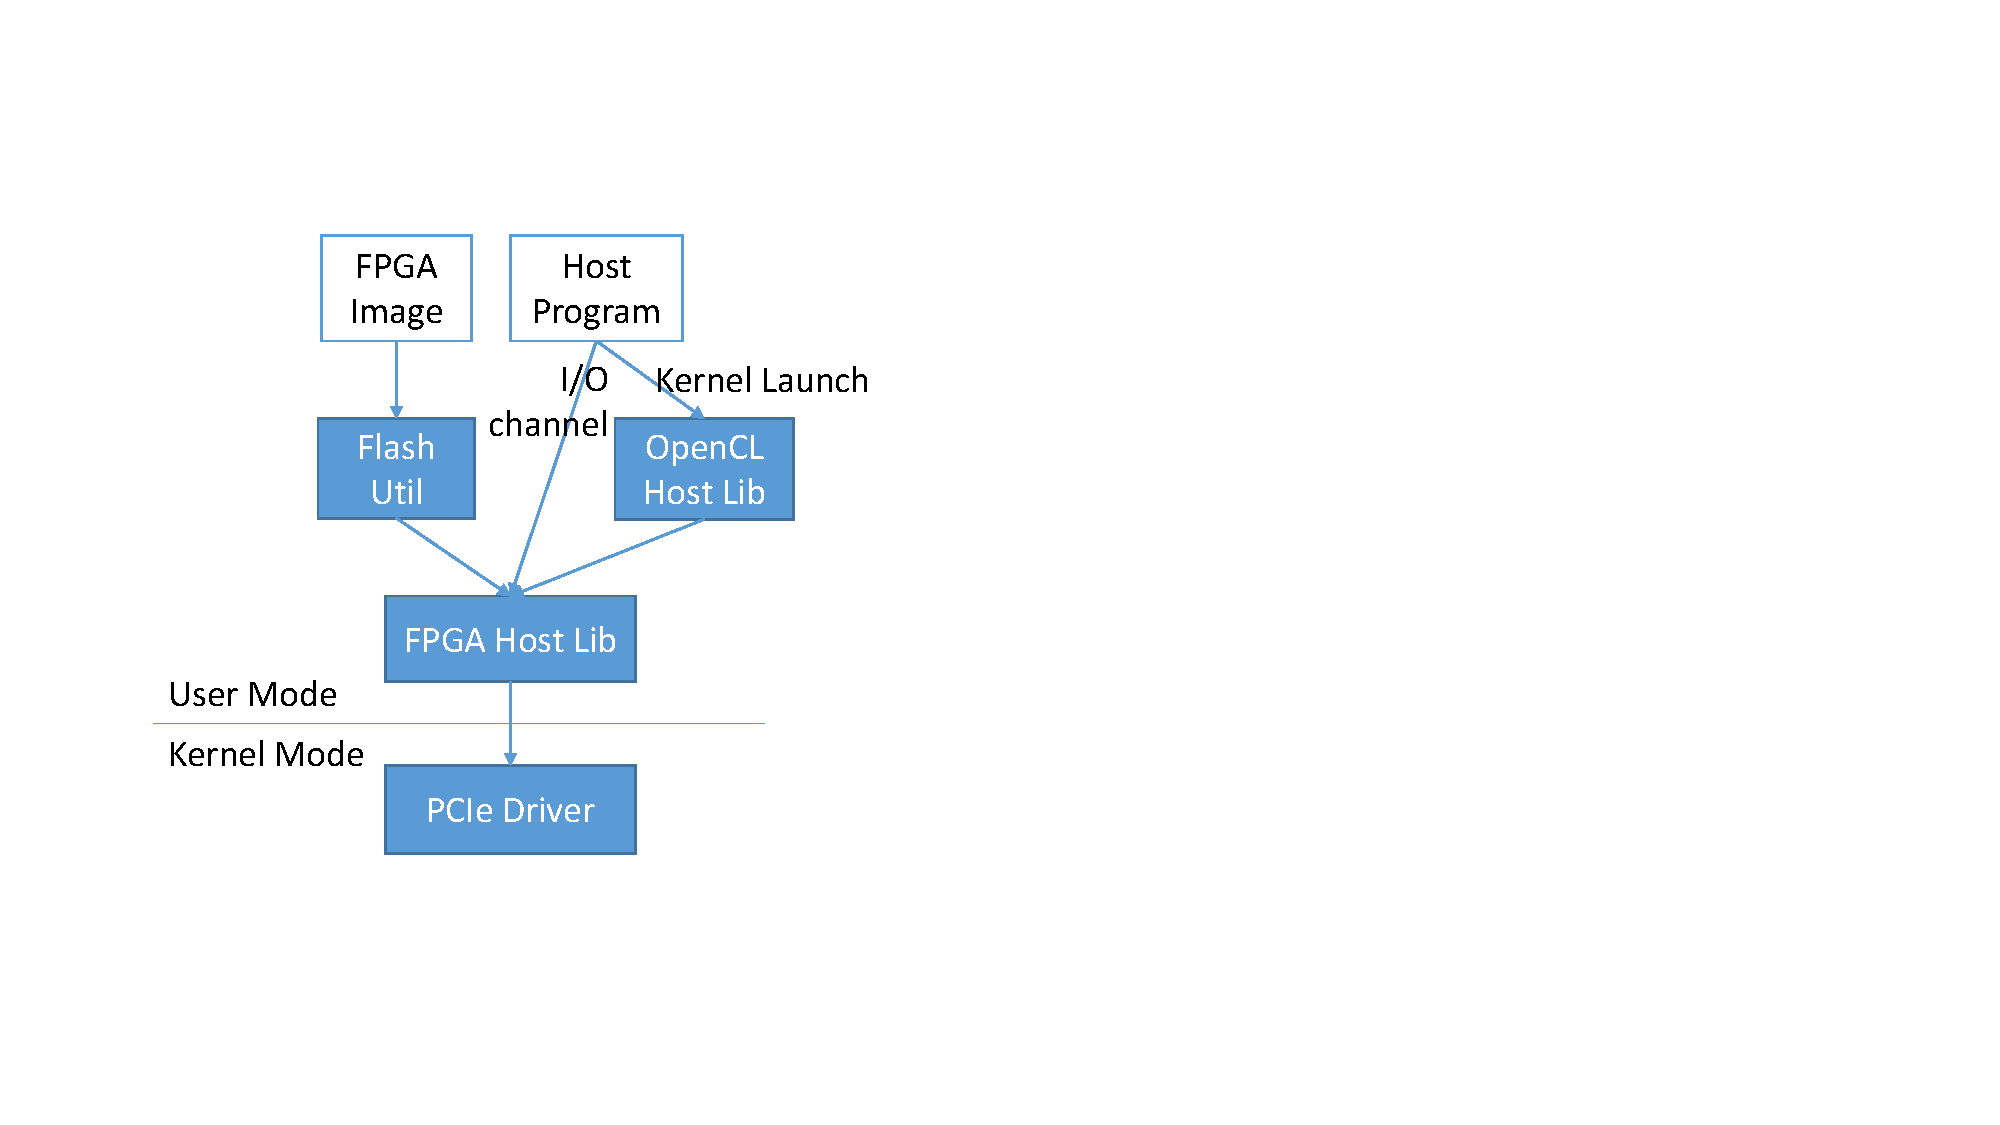
\includegraphics[width=0.8\columnwidth]{image/CatapultRuntime}
	\vspace{-0.15in}
	\caption{ClickNP Runtime Architecture}
	\vspace{-0.15in}
	\label{fig:CatapultFPGAArch}
	%    \vspace{-2mm}
\end{figure}
}
